%!TEX root = Thesis_main.tex

\chapter{Results}
\label{chapter7}
\section{Simulations results}
The goal of the initial simulations is to assess the actual convenience of our approach and to tune the MPC parameters and weights. Once achieved good performances with a proper set of parameters, the controller can betested with the physical system.\\
Initially some simulations with only the mobile base have been run on a trajectory with low-radius curves (in Figure \ref{traj_base_curves}), seeing the effect of different control horizon lengths and of input disturbances. This trajectory has been chosen to simulate the system going around some 
\begin{figure}[h!]
\centering
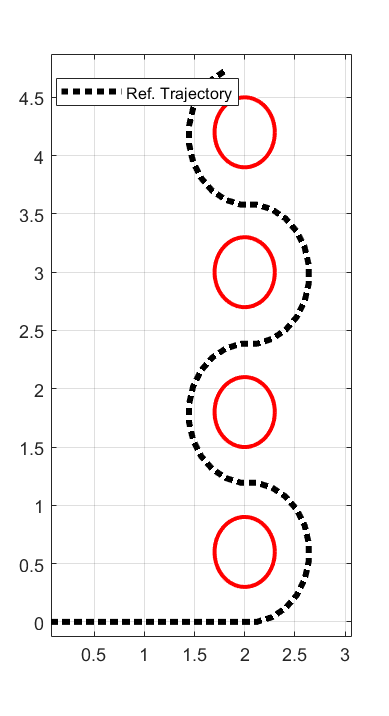
\includegraphics[scale=0.4]{traj_base_curves}
\caption{Base trajectory for simulations: radius=0.6m}
\label{traj_base_curves}
\end{figure}
As it is possible to see from Figures \ref{base_curves} and \ref{base_curves_errors}, our controller is able to manage even high disturbances, but because of the limitation introduced by the parameterization of the input, it is more difficult for the optimizer to find a curve built on polynomial input that correctly approximates the given trajectory. This effect is even enlarged by the weighting profile of the cost function which give less importance to the accuracy of the first steps in the control horizon. Nevertheless Figure \ref{base_curves_errors} let us see that the time elapsed during the the optimization process doesn't increase exponentially like in traditional MPC, but it stays almost constant.
\begin{figure}[h!]
	\centering
	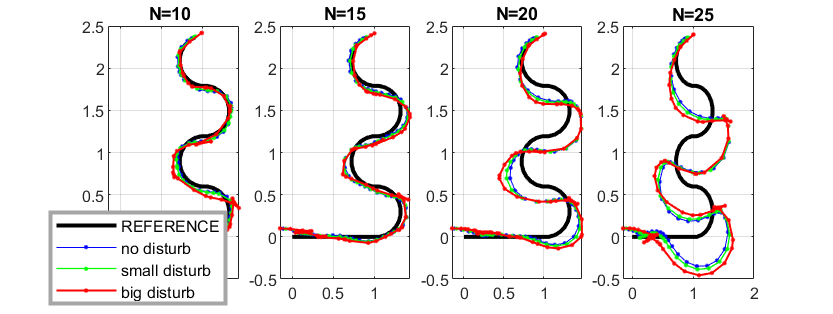
\includegraphics[scale=0.36]{base_curves_small.png}
	\caption{Mobile platform trajectories with different N}
	\label{base_curves}
\end{figure}
%\begin{figure}[h!]
%	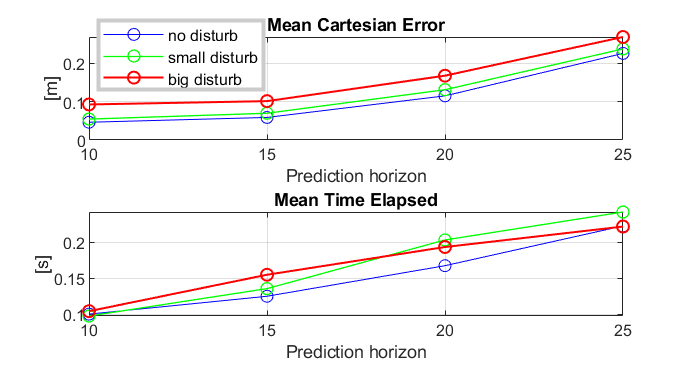
\includegraphics[scale=0.45]{images/base_curves_errorsandtime.png}
%	\caption{Optimization time and Cartesian error when varying N}
%	\label{base_curves_errors}
%\end{figure}
Then the motion of the entire MM has been simulated performing an EE position and orientation trajectory tracking on a sinusoidal 3D path, allowing us to more accurately tune some parameters. 
We compared the solving times of our approach with the ones of a traditional MPC dealing with the same problem at different time horizon, in Figure \ref{solving_times}. It is easy to see the convenience of our approach, since the number of the unknowns that the optimizer has to find does not increase with $N$ and so with the dimension of the problem. In other words the mean time needed to the optimizer to solve the MPC problem stays almost constant instead of increasing exponentially.
%\begin{figure}[h!]
%	\centering
%	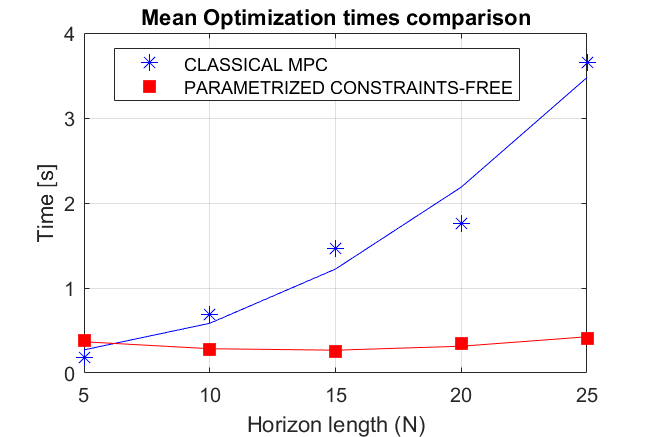
\includegraphics[scale=0.40]{images/solving_times_small.png}
%	\caption{Solving time comparison}
%	\label{solving_times}
%\end{figure}
However, from the results showed in Figure \ref{ee_tests} and from other experiments run with different time steps $T$, it can be seen that, as in previous tests, the biggest limit of this controller is that it cannot find a trajectory defined with polynomial inputs that can stay close to too complex desired trajectories during long prediction horizons

Considerazioni iniziali sulle traiettorie provate e perchè abbiamo scelto tali traiettorie (farei step e traiettoria grasping)
	\subsection{effect of N}
		
	\subsection{effect of different parameterization}
		
	\subsection{Movement of the system toward grasping area}
 ... Parameterization for the control input of the base as well as the parameterization for the UR5 joints have been done according to the smoothness of the trajectory to be tracked and the number of desired points belonging to these trajectories. In particular the base parameterization has been chosen polynomial quadratic, while two choice of parameterization have been done for the arm joints: linear and constant. The effect of this choice will be discussed later on. 
		\subsubsection{errors in tracking}
			
		\subsubsection{time elapsed}
			comparison con clasical MPC logic
		\subsubsection{J function components}

	\subsection{Trajectory tracking in grasping operation}

		\subsubsection{errors in tracking}
			
		\subsubsection{time elapsed}
			comparison con clasical MPC logic
		\subsubsection{J function components}
		
		\subsection{passaggio da una funz costo all'altra}
	
\section{Physical experiments results}
	parlare del posizionamento della base che non funziona bene ad alte velocità e si possono mettere anche dei grafici per la ripetibilità della base e una foto
	parlare del sistema di telecamere che è stato usato ma non funzionava bene in termini di stabilità e magari mettere qualche foto?
	\subsection{Movement of the system toward grasping area}

		\subsubsection{errors in tracking}
			
		\subsubsection{time elapsed}
			comparison con clasical MPC logic

	\subsection{Trajectory tracking in grasping operation}

	The controller has been tested to perform grasping operations tracking EE trajectories as position and orientation in time as well as a desired motion of the base. For these experiments the system shows a response comparable to the model used in simulation. Anyway, considering the errors due to the positioning system of the base as mentioned before, did not allow to test the system at high speed. The time chosen to perform this task has been setted between $35$ and $45 s$ according to the choice of $T_k$. 


	\begin{table}[]
	
	\centering

	\begin{tabular}{|l|l|l|ll}
	\cline{1-2}
	\multicolumn{2}{|l|}{ \textbf{Parameters} }	\\ \cline{1-2}
	$N$     				&  $10$ 	      					\\ \cline{1-2}
	$T$     				&  $0.4\ s$  	      					\\ \cline{1-2}
	$m$     				&  $3$ 	      						\\ \cline{1-2}
	$w_1$    				&  $1e6$       						\\ \cline{1-2}
	$w_2$    				&  $50$       						\\ \cline{1-2}
	$w_3$    				&  $1e5$       						\\ \cline{1-2}
	$w_4$    				&  $5e3$       						\\ \cline{1-2}
	$w_5$    				&  $0$      						\\ \cline{1-2}
	\end{tabular}
	\quad
	\begin{tabular}{|l|l|l|ll}
	\cline{1-3}
	\textbf{Constraints}    	& \textbf{min} 					& \textbf{max}			\\ \cline{1-3}
	$x$		 			 		&  -0.15 $m$ 					&  3.00 $m$ 			\\ \cline{1-3}
	$x$		 			 		&  -2.60 $m$ 					&  0.20 $m$ 			\\ \cline{1-3}
	$\Theta$ 			 		&  -$\infty$  					&  +$\infty$ 			\\ \cline{1-3}
	$\Theta_1$ (Base)			&  -350°  						&  350° 				\\ \cline{1-3}
	$\Theta_2$ (Shoulder)		&  -180° 						&  0°		 			\\ \cline{1-3}
	$\Theta_3$ (Elbow) 			&  -140° 						&  140°		 			\\ \cline{1-3}
	$\Theta_4$ (Wrist1) 		&  -180° 						&  0°		 			\\ \cline{1-3}
	$\Theta_5$ (Wrist2)			&  -140° 						&  97°		 			\\ \cline{1-3} 
	$\Theta_6$ (Wrist3) 		&  -357° 						&  357°		 			\\ \cline{1-3}
	$\dot{v}$ 			 		&  -0.1 $m/s^2$					&  -0.1 $m/s^2$ 		\\ \cline{1-3}
	$\dot{\omega}$		 		&  -0.1 $rad/s^2$ 				&  -0.1 $rad/s^2$		\\ \cline{1-3}
	$\dot{\Theta}_{1,\dots,6}$	&  -0.2 $rad/s$					&  -0.2 $rad/s$ 		\\ \cline{1-3}
	\end{tabular}
	\caption{Experiment Parameters}
	\label{tableparam1}
	\end{table}

	Parameterization has been chosen as in simulation, so comparing linear and constant parameterization for the arm joints. The gripper used in the experiments is a Robotiq 2-Finger 85mm for Universal Robots. The instant at which the gripper has to be closed was defined offline and the communication ensured through a ROS node. The first experiment results, performed with a linear parameterization for the arm joints are obtained using the parameters shown in Table \ref{tableparam1}. 
	In Figure \ref{traj_ee1} the performed trajectory is shown. The result is then compared in Figure \ref{traj_ee1_comp} with the trajectory performed in simulation. 

	\begin{figure}[h!]
	\centering
	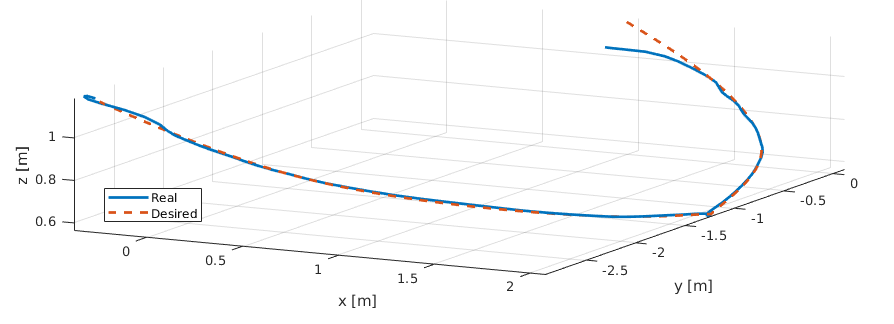
\includegraphics[scale=0.36]{traj_ee1.png}
	\caption{EE Position during grasping}
	\label{traj_ee1}
	\end{figure}
		\subsubsection{errors in tracking}
			
		\subsubsection{time elapsed}
			comparison con clasical MPC logic
		\subsubsection{J function components}
